\documentclass{standalone}
\usepackage{tikz}
\usetikzlibrary{patterns, positioning}

\begin{document}
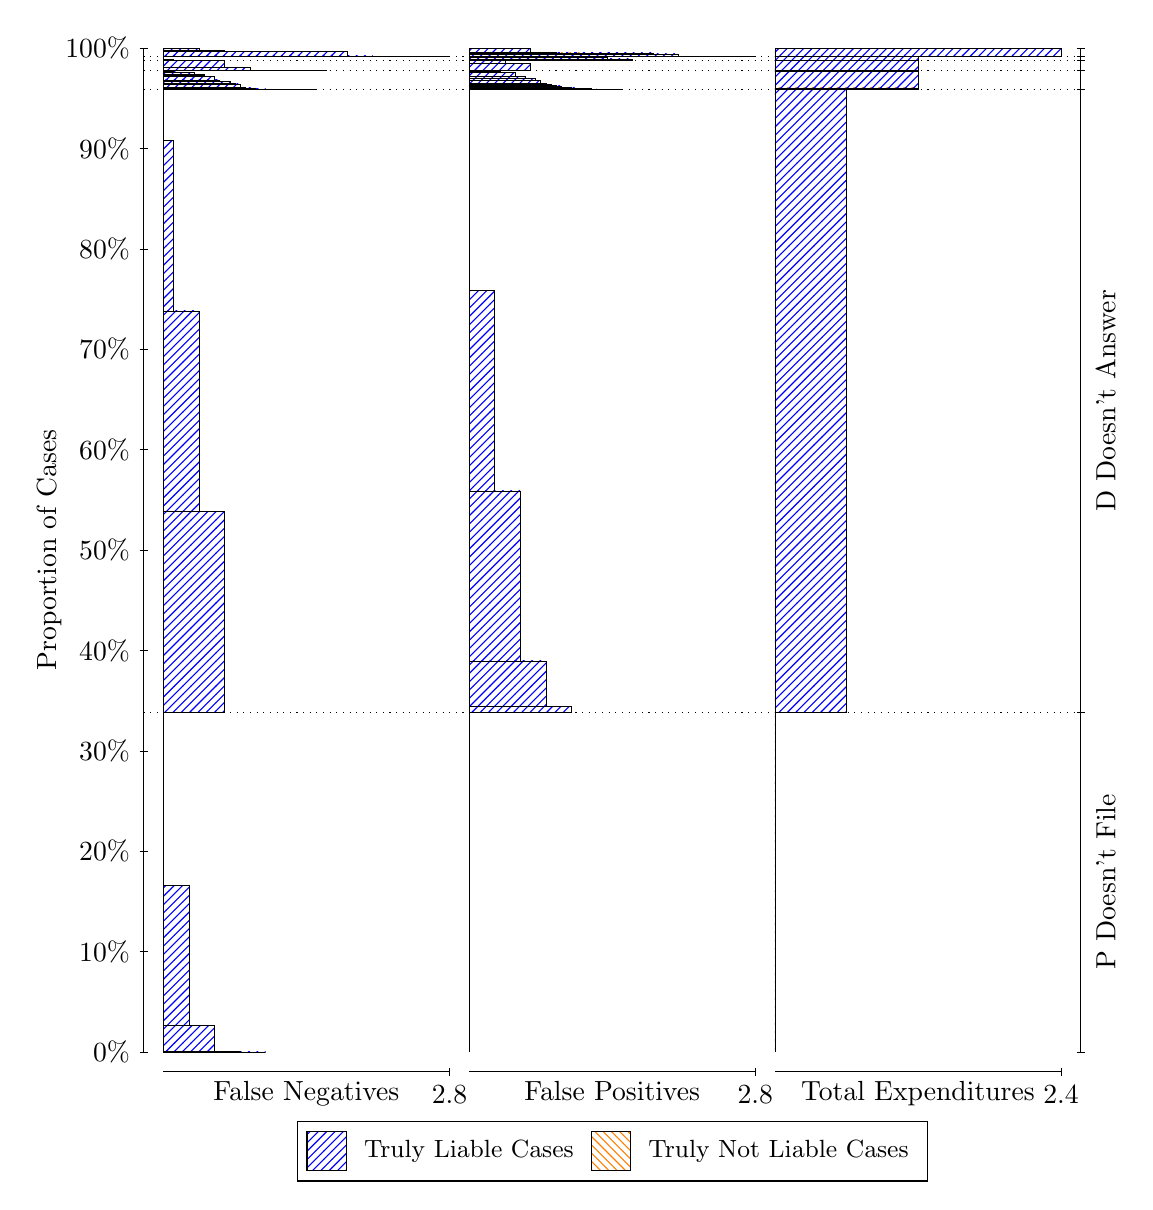
\begin{tikzpicture}
\draw[black, very thin] (1.5,1.75) -- (1.5,14.5);
\node[rotate=90, anchor=center] at (0.3, 8.125) {Proportion of Cases};
\draw[black, very thin] (1.45,1.75) -- (1.55,1.75);
\node[anchor=east] at (1.45, 1.75) {0\%};
\draw[black, very thin] (1.45,3.025) -- (1.55,3.025);
\node[anchor=east] at (1.45, 3.025) {10\%};
\draw[black, very thin] (1.45,4.3) -- (1.55,4.3);
\node[anchor=east] at (1.45, 4.3) {20\%};
\draw[black, very thin] (1.45,5.575) -- (1.55,5.575);
\node[anchor=east] at (1.45, 5.575) {30\%};
\draw[black, very thin] (1.45,6.85) -- (1.55,6.85);
\node[anchor=east] at (1.45, 6.85) {40\%};
\draw[black, very thin] (1.45,8.125) -- (1.55,8.125);
\node[anchor=east] at (1.45, 8.125) {50\%};
\draw[black, very thin] (1.45,9.4) -- (1.55,9.4);
\node[anchor=east] at (1.45, 9.4) {60\%};
\draw[black, very thin] (1.45,10.675) -- (1.55,10.675);
\node[anchor=east] at (1.45, 10.675) {70\%};
\draw[black, very thin] (1.45,11.95) -- (1.55,11.95);
\node[anchor=east] at (1.45, 11.95) {80\%};
\draw[black, very thin] (1.45,13.225) -- (1.55,13.225);
\node[anchor=east] at (1.45, 13.225) {90\%};
\draw[black, very thin] (1.45,14.5) -- (1.55,14.5);
\node[anchor=east] at (1.45, 14.5) {100\%};

\draw[black, very thin] (13.4,1.75) -- (13.4,14.5);
\draw[black, very thin] (13.35,1.75) -- (13.45,1.75);
\node[anchor=west] at (13.35, 1.75) {};
\draw[black, very thin] (13.35,6.0661) -- (13.45,6.0661);
\node[anchor=west] at (13.35, 6.0661) {};
\draw[black, very thin] (13.35,13.973) -- (13.45,13.973);
\node[anchor=west] at (13.35, 13.973) {};
\draw[black, very thin] (13.35,14.214) -- (13.45,14.214);
\node[anchor=west] at (13.35, 14.214) {};
\draw[black, very thin] (13.35,14.347) -- (13.45,14.347);
\node[anchor=west] at (13.35, 14.347) {};
\draw[black, very thin] (13.35,14.394) -- (13.45,14.394);
\node[anchor=west] at (13.35, 14.394) {};
\draw[black, very thin] (13.35,14.5) -- (13.45,14.5);
\node[anchor=west] at (13.35, 14.5) {};

\draw[black, very thin, pattern color=blue, pattern=north east lines] (1.75,1.75) rectangle (3.0476,1.75);
\draw[black, very thin, pattern color=blue, pattern=north east lines] (1.75,1.75) rectangle (2.7232,1.7528);
\draw[black, very thin, pattern color=blue, pattern=north east lines] (1.75,1.7528) rectangle (2.3988,2.0841);
\draw[black, very thin, pattern color=blue, pattern=north east lines] (1.75,2.0841) rectangle (2.0744,3.8627);
\draw[black, very thin, pattern color=orange, pattern=north west lines] (1.75,3.8627) rectangle (1.75,3.8627);
\draw[black, very thin, pattern color=blue, pattern=north east lines] (1.75,3.8627) rectangle (1.75,6.0661);
\draw[black, very thin, pattern color=blue, pattern=north east lines] (1.75,6.0661) rectangle (2.5286,8.616);
\draw[black, very thin, pattern color=blue, pattern=north east lines] (1.75,8.616) rectangle (2.2042,11.163);
\draw[black, very thin, pattern color=blue, pattern=north east lines] (1.75,11.163) rectangle (1.8798,13.323);
\draw[black, very thin, pattern color=orange, pattern=north west lines] (1.75,13.323) rectangle (1.75,13.323);
\draw[black, very thin, pattern color=blue, pattern=north east lines] (1.75,13.323) rectangle (1.75,13.973);
\draw[black, very thin, pattern color=blue, pattern=north east lines] (1.75,13.973) rectangle (3.6964,13.973);
\draw[black, very thin, pattern color=blue, pattern=north east lines] (1.75,13.973) rectangle (3.5667,13.973);
\draw[black, very thin, pattern color=blue, pattern=north east lines] (1.75,13.973) rectangle (3.4369,13.973);
\draw[black, very thin, pattern color=blue, pattern=north east lines] (1.75,13.973) rectangle (3.372,13.973);
\draw[black, very thin, pattern color=blue, pattern=north east lines] (1.75,13.973) rectangle (3.3071,13.973);
\draw[black, very thin, pattern color=blue, pattern=north east lines] (1.75,13.973) rectangle (3.2423,13.973);
\draw[black, very thin, pattern color=blue, pattern=north east lines] (1.75,13.973) rectangle (3.1774,13.973);
\draw[black, very thin, pattern color=blue, pattern=north east lines] (1.75,13.973) rectangle (3.1125,13.973);
\draw[black, very thin, pattern color=blue, pattern=north east lines] (1.75,13.973) rectangle (3.0476,13.982);
\draw[black, very thin, pattern color=blue, pattern=north east lines] (1.75,13.982) rectangle (2.9827,13.982);
\draw[black, very thin, pattern color=blue, pattern=north east lines] (1.75,13.982) rectangle (2.9179,13.982);
\draw[black, very thin, pattern color=blue, pattern=north east lines] (1.75,13.982) rectangle (2.9179,13.994);
\draw[black, very thin, pattern color=blue, pattern=north east lines] (1.75,13.994) rectangle (2.853,13.994);
\draw[black, very thin, pattern color=blue, pattern=north east lines] (1.75,13.994) rectangle (2.7881,14.001);
\draw[black, very thin, pattern color=blue, pattern=north east lines] (1.75,14.001) rectangle (2.7881,14.001);
\draw[black, very thin, pattern color=blue, pattern=north east lines] (1.75,14.001) rectangle (2.7232,14.045);
\draw[black, very thin, pattern color=blue, pattern=north east lines] (1.75,14.045) rectangle (2.6583,14.048);
\draw[black, very thin, pattern color=blue, pattern=north east lines] (1.75,14.048) rectangle (2.5935,14.048);
\draw[black, very thin, pattern color=blue, pattern=north east lines] (1.75,14.048) rectangle (2.5935,14.072);
\draw[black, very thin, pattern color=blue, pattern=north east lines] (1.75,14.072) rectangle (2.5286,14.077);
\draw[black, very thin, pattern color=blue, pattern=north east lines] (1.75,14.077) rectangle (2.4637,14.095);
\draw[black, very thin, pattern color=blue, pattern=north east lines] (1.75,14.095) rectangle (2.4637,14.095);
\draw[black, very thin, pattern color=blue, pattern=north east lines] (1.75,14.095) rectangle (2.3988,14.14);
\draw[black, very thin, pattern color=blue, pattern=north east lines] (1.75,14.14) rectangle (2.3339,14.144);
\draw[black, very thin, pattern color=blue, pattern=north east lines] (1.75,14.144) rectangle (2.3339,14.147);
\draw[black, very thin, pattern color=blue, pattern=north east lines] (1.75,14.147) rectangle (2.269,14.149);
\draw[black, very thin, pattern color=blue, pattern=north east lines] (1.75,14.149) rectangle (2.269,14.161);
\draw[black, very thin, pattern color=blue, pattern=north east lines] (1.75,14.161) rectangle (2.2042,14.17);
\draw[black, very thin, pattern color=blue, pattern=north east lines] (1.75,14.17) rectangle (2.1393,14.187);
\draw[black, very thin, pattern color=blue, pattern=north east lines] (1.75,14.187) rectangle (2.1393,14.187);
\draw[black, very thin, pattern color=blue, pattern=north east lines] (1.75,14.187) rectangle (2.0744,14.191);
\draw[black, very thin, pattern color=blue, pattern=north east lines] (1.75,14.191) rectangle (2.0095,14.193);
\draw[black, very thin, pattern color=blue, pattern=north east lines] (1.75,14.193) rectangle (2.0095,14.195);
\draw[black, very thin, pattern color=blue, pattern=north east lines] (1.75,14.195) rectangle (1.9446,14.198);
\draw[black, very thin, pattern color=blue, pattern=north east lines] (1.75,14.198) rectangle (1.8798,14.203);
\draw[black, very thin, pattern color=blue, pattern=north east lines] (1.75,14.203) rectangle (1.8149,14.204);
\draw[black, very thin, pattern color=orange, pattern=north west lines] (1.75,14.204) rectangle (1.75,14.204);
\draw[black, very thin, pattern color=blue, pattern=north east lines] (1.75,14.204) rectangle (1.75,14.214);
\draw[black, very thin, pattern color=blue, pattern=north east lines] (1.75,14.214) rectangle (3.8262,14.214);
\draw[black, very thin, pattern color=blue, pattern=north east lines] (1.75,14.214) rectangle (3.5018,14.214);
\draw[black, very thin, pattern color=blue, pattern=north east lines] (1.75,14.214) rectangle (3.1774,14.219);
\draw[black, very thin, pattern color=blue, pattern=north east lines] (1.75,14.219) rectangle (2.853,14.256);
\draw[black, very thin, pattern color=blue, pattern=north east lines] (1.75,14.256) rectangle (2.5286,14.347);
\draw[black, very thin, pattern color=orange, pattern=north west lines] (1.75,14.347) rectangle (1.75,14.347);
\draw[black, very thin, pattern color=blue, pattern=north east lines] (1.75,14.347) rectangle (2.5286,14.347);
\draw[black, very thin, pattern color=blue, pattern=north east lines] (1.75,14.347) rectangle (2.2042,14.347);
\draw[black, very thin, pattern color=blue, pattern=north east lines] (1.75,14.347) rectangle (1.8798,14.358);
\draw[black, very thin, pattern color=orange, pattern=north west lines] (1.75,14.358) rectangle (1.75,14.358);
\draw[black, very thin, pattern color=blue, pattern=north east lines] (1.75,14.358) rectangle (1.75,14.394);
\draw[black, very thin, pattern color=blue, pattern=north east lines] (1.75,14.394) rectangle (5.3833,14.394);
\draw[black, very thin, pattern color=blue, pattern=north east lines] (1.75,14.394) rectangle (5.0589,14.394);
\draw[black, very thin, pattern color=blue, pattern=north east lines] (1.75,14.394) rectangle (4.7345,14.394);
\draw[black, very thin, pattern color=blue, pattern=north east lines] (1.75,14.394) rectangle (4.4101,14.401);
\draw[black, very thin, pattern color=blue, pattern=north east lines] (1.75,14.401) rectangle (4.0857,14.454);
\draw[black, very thin, pattern color=blue, pattern=north east lines] (1.75,14.454) rectangle (3.7613,14.457);
\draw[black, very thin, pattern color=blue, pattern=north east lines] (1.75,14.457) rectangle (3.5018,14.457);
\draw[black, very thin, pattern color=blue, pattern=north east lines] (1.75,14.457) rectangle (3.4369,14.457);
\draw[black, very thin, pattern color=blue, pattern=north east lines] (1.75,14.457) rectangle (3.1774,14.457);
\draw[black, very thin, pattern color=blue, pattern=north east lines] (1.75,14.457) rectangle (2.853,14.457);
\draw[black, very thin, pattern color=blue, pattern=north east lines] (1.75,14.457) rectangle (2.5286,14.47);
\draw[black, very thin, pattern color=blue, pattern=north east lines] (1.75,14.47) rectangle (2.2042,14.497);
\draw[black, very thin, pattern color=blue, pattern=north east lines] (1.75,14.497) rectangle (1.8798,14.5);
\draw[black, very thin, pattern color=orange, pattern=north west lines] (1.75,14.5) rectangle (1.75,14.5);
\draw[black, very thin, pattern color=blue, pattern=north east lines] (1.75,14.5) rectangle (1.75,14.5);
\draw[black, very thin, pattern color=orange, pattern=north west lines] (5.6333,1.75) rectangle (5.6333,1.75);
\draw[black, very thin, pattern color=blue, pattern=north east lines] (5.6333,1.75) rectangle (5.6333,6.0661);
\draw[black, very thin, pattern color=orange, pattern=north west lines] (5.6333,6.0661) rectangle (6.931,6.0661);
\draw[black, very thin, pattern color=blue, pattern=north east lines] (5.6333,6.0661) rectangle (6.931,6.141);
\draw[black, very thin, pattern color=blue, pattern=north east lines] (5.6333,6.141) rectangle (6.6065,6.7161);
\draw[black, very thin, pattern color=blue, pattern=north east lines] (5.6333,6.7161) rectangle (6.2821,8.8768);
\draw[black, very thin, pattern color=blue, pattern=north east lines] (5.6333,8.8768) rectangle (5.9577,11.423);
\draw[black, very thin, pattern color=blue, pattern=north east lines] (5.6333,11.423) rectangle (5.6333,13.973);
\draw[black, very thin, pattern color=orange, pattern=north west lines] (5.6333,13.973) rectangle (7.5798,13.973);
\draw[black, very thin, pattern color=blue, pattern=north east lines] (5.6333,13.973) rectangle (7.5798,13.975);
\draw[black, very thin, pattern color=orange, pattern=north west lines] (5.6333,13.975) rectangle (7.45,13.975);
\draw[black, very thin, pattern color=blue, pattern=north east lines] (5.6333,13.975) rectangle (7.45,13.976);
\draw[black, very thin, pattern color=orange, pattern=north west lines] (5.6333,13.976) rectangle (7.3202,13.976);
\draw[black, very thin, pattern color=blue, pattern=north east lines] (5.6333,13.976) rectangle (7.3202,13.979);
\draw[black, very thin, pattern color=blue, pattern=north east lines] (5.6333,13.979) rectangle (7.2554,13.98);
\draw[black, very thin, pattern color=orange, pattern=north west lines] (5.6333,13.98) rectangle (7.1905,13.98);
\draw[black, very thin, pattern color=blue, pattern=north east lines] (5.6333,13.98) rectangle (7.1905,13.983);
\draw[black, very thin, pattern color=blue, pattern=north east lines] (5.6333,13.983) rectangle (7.1256,13.984);
\draw[black, very thin, pattern color=orange, pattern=north west lines] (5.6333,13.984) rectangle (7.0607,13.984);
\draw[black, very thin, pattern color=blue, pattern=north east lines] (5.6333,13.984) rectangle (7.0607,13.99);
\draw[black, very thin, pattern color=blue, pattern=north east lines] (5.6333,13.99) rectangle (6.9958,13.993);
\draw[black, very thin, pattern color=orange, pattern=north west lines] (5.6333,13.993) rectangle (6.931,13.993);
\draw[black, very thin, pattern color=blue, pattern=north east lines] (5.6333,13.993) rectangle (6.931,13.997);
\draw[black, very thin, pattern color=blue, pattern=north east lines] (5.6333,13.997) rectangle (6.8661,14.001);
\draw[black, very thin, pattern color=orange, pattern=north west lines] (5.6333,14.001) rectangle (6.8012,14.001);
\draw[black, very thin, pattern color=blue, pattern=north east lines] (5.6333,14.001) rectangle (6.8012,14.018);
\draw[black, very thin, pattern color=blue, pattern=north east lines] (5.6333,14.018) rectangle (6.7363,14.027);
\draw[black, very thin, pattern color=orange, pattern=north west lines] (5.6333,14.027) rectangle (6.6714,14.027);
\draw[black, very thin, pattern color=blue, pattern=north east lines] (5.6333,14.027) rectangle (6.6714,14.039);
\draw[black, very thin, pattern color=blue, pattern=north east lines] (5.6333,14.039) rectangle (6.6714,14.041);
\draw[black, very thin, pattern color=blue, pattern=north east lines] (5.6333,14.041) rectangle (6.6065,14.048);
\draw[black, very thin, pattern color=orange, pattern=north west lines] (5.6333,14.048) rectangle (6.5417,14.048);
\draw[black, very thin, pattern color=blue, pattern=north east lines] (5.6333,14.048) rectangle (6.5417,14.092);
\draw[black, very thin, pattern color=blue, pattern=north east lines] (5.6333,14.092) rectangle (6.4768,14.11);
\draw[black, very thin, pattern color=blue, pattern=north east lines] (5.6333,14.11) rectangle (6.4119,14.116);
\draw[black, very thin, pattern color=blue, pattern=north east lines] (5.6333,14.116) rectangle (6.347,14.14);
\draw[black, very thin, pattern color=blue, pattern=north east lines] (5.6333,14.14) rectangle (6.347,14.14);
\draw[black, very thin, pattern color=blue, pattern=north east lines] (5.6333,14.14) rectangle (6.2821,14.143);
\draw[black, very thin, pattern color=blue, pattern=north east lines] (5.6333,14.143) rectangle (6.2173,14.187);
\draw[black, very thin, pattern color=blue, pattern=north east lines] (5.6333,14.187) rectangle (6.1524,14.194);
\draw[black, very thin, pattern color=blue, pattern=north east lines] (5.6333,14.194) rectangle (6.0875,14.194);
\draw[black, very thin, pattern color=blue, pattern=north east lines] (5.6333,14.194) rectangle (6.0226,14.206);
\draw[black, very thin, pattern color=blue, pattern=north east lines] (5.6333,14.206) rectangle (6.0226,14.206);
\draw[black, very thin, pattern color=blue, pattern=north east lines] (5.6333,14.206) rectangle (5.9577,14.206);
\draw[black, very thin, pattern color=blue, pattern=north east lines] (5.6333,14.206) rectangle (5.8929,14.214);
\draw[black, very thin, pattern color=blue, pattern=north east lines] (5.6333,14.214) rectangle (5.828,14.214);
\draw[black, very thin, pattern color=blue, pattern=north east lines] (5.6333,14.214) rectangle (5.7631,14.214);
\draw[black, very thin, pattern color=blue, pattern=north east lines] (5.6333,14.214) rectangle (5.6982,14.214);
\draw[black, very thin, pattern color=blue, pattern=north east lines] (5.6333,14.214) rectangle (5.6333,14.214);
\draw[black, very thin, pattern color=orange, pattern=north west lines] (5.6333,14.214) rectangle (6.4119,14.214);
\draw[black, very thin, pattern color=blue, pattern=north east lines] (5.6333,14.214) rectangle (6.4119,14.305);
\draw[black, very thin, pattern color=blue, pattern=north east lines] (5.6333,14.305) rectangle (6.0875,14.342);
\draw[black, very thin, pattern color=blue, pattern=north east lines] (5.6333,14.342) rectangle (5.7631,14.347);
\draw[black, very thin, pattern color=blue, pattern=north east lines] (5.6333,14.347) rectangle (5.6333,14.347);
\draw[black, very thin, pattern color=orange, pattern=north west lines] (5.6333,14.347) rectangle (7.7095,14.347);
\draw[black, very thin, pattern color=blue, pattern=north east lines] (5.6333,14.347) rectangle (7.7095,14.362);
\draw[black, very thin, pattern color=blue, pattern=north east lines] (5.6333,14.362) rectangle (7.3851,14.383);
\draw[black, very thin, pattern color=blue, pattern=north east lines] (5.6333,14.383) rectangle (7.0607,14.394);
\draw[black, very thin, pattern color=blue, pattern=north east lines] (5.6333,14.394) rectangle (6.7363,14.394);
\draw[black, very thin, pattern color=blue, pattern=north east lines] (5.6333,14.394) rectangle (6.4119,14.394);
\draw[black, very thin, pattern color=orange, pattern=north west lines] (5.6333,14.394) rectangle (9.2667,14.394);
\draw[black, very thin, pattern color=blue, pattern=north east lines] (5.6333,14.394) rectangle (9.2667,14.394);
\draw[black, very thin, pattern color=orange, pattern=north west lines] (5.6333,14.394) rectangle (8.9423,14.394);
\draw[black, very thin, pattern color=blue, pattern=north east lines] (5.6333,14.394) rectangle (8.9423,14.394);
\draw[black, very thin, pattern color=orange, pattern=north west lines] (5.6333,14.394) rectangle (8.6179,14.394);
\draw[black, very thin, pattern color=blue, pattern=north east lines] (5.6333,14.394) rectangle (8.6179,14.397);
\draw[black, very thin, pattern color=orange, pattern=north west lines] (5.6333,14.397) rectangle (8.2935,14.397);
\draw[black, very thin, pattern color=blue, pattern=north east lines] (5.6333,14.397) rectangle (8.2935,14.425);
\draw[black, very thin, pattern color=blue, pattern=north east lines] (5.6333,14.425) rectangle (7.969,14.437);
\draw[black, very thin, pattern color=blue, pattern=north east lines] (5.6333,14.437) rectangle (7.6446,14.438);
\draw[black, very thin, pattern color=blue, pattern=north east lines] (5.6333,14.438) rectangle (7.3202,14.438);
\draw[black, very thin, pattern color=orange, pattern=north west lines] (5.6333,14.438) rectangle (7.0607,14.438);
\draw[black, very thin, pattern color=blue, pattern=north east lines] (5.6333,14.438) rectangle (7.0607,14.438);
\draw[black, very thin, pattern color=blue, pattern=north east lines] (5.6333,14.438) rectangle (6.9958,14.438);
\draw[black, very thin, pattern color=blue, pattern=north east lines] (5.6333,14.438) rectangle (6.7363,14.438);
\draw[black, very thin, pattern color=orange, pattern=north west lines] (5.6333,14.438) rectangle (6.7363,14.438);
\draw[black, very thin, pattern color=blue, pattern=north east lines] (5.6333,14.438) rectangle (6.7363,14.441);
\draw[black, very thin, pattern color=blue, pattern=north east lines] (5.6333,14.441) rectangle (6.4119,14.441);
\draw[black, very thin, pattern color=orange, pattern=north west lines] (5.6333,14.441) rectangle (6.4119,14.441);
\draw[black, very thin, pattern color=blue, pattern=north east lines] (5.6333,14.441) rectangle (6.4119,14.493);
\draw[black, very thin, pattern color=blue, pattern=north east lines] (5.6333,14.493) rectangle (6.0875,14.493);
\draw[black, very thin, pattern color=blue, pattern=north east lines] (5.6333,14.493) rectangle (6.0875,14.5);
\draw[black, very thin, pattern color=blue, pattern=north east lines] (5.6333,14.5) rectangle (5.7631,14.5);
\draw[black, very thin, pattern color=blue, pattern=north east lines] (5.6333,14.5) rectangle (5.7631,14.5);
\draw[black, very thin, pattern color=blue, pattern=north east lines] (5.6333,14.5) rectangle (5.6333,14.5);
\draw[black, very thin, pattern color=orange, pattern=north west lines] (9.5167,1.75) rectangle (9.5167,1.75);
\draw[black, very thin, pattern color=blue, pattern=north east lines] (9.5167,1.75) rectangle (9.5167,6.0661);
\draw[black, very thin, pattern color=orange, pattern=north west lines] (9.5167,6.0661) rectangle (10.425,6.0661);
\draw[black, very thin, pattern color=blue, pattern=north east lines] (9.5167,6.0661) rectangle (10.425,13.973);
\draw[black, very thin, pattern color=orange, pattern=north west lines] (9.5167,13.973) rectangle (11.333,13.973);
\draw[black, very thin, pattern color=blue, pattern=north east lines] (9.5167,13.973) rectangle (11.333,13.993);
\draw[black, very thin, pattern color=orange, pattern=north west lines] (9.5167,13.993) rectangle (11.333,13.993);
\draw[black, very thin, pattern color=blue, pattern=north east lines] (9.5167,13.993) rectangle (11.333,14.205);
\draw[black, very thin, pattern color=orange, pattern=north west lines] (9.5167,14.205) rectangle (11.333,14.205);
\draw[black, very thin, pattern color=blue, pattern=north east lines] (9.5167,14.205) rectangle (11.333,14.214);
\draw[black, very thin, pattern color=orange, pattern=north west lines] (9.5167,14.214) rectangle (11.333,14.214);
\draw[black, very thin, pattern color=blue, pattern=north east lines] (9.5167,14.214) rectangle (11.333,14.347);
\draw[black, very thin, pattern color=orange, pattern=north west lines] (9.5167,14.347) rectangle (11.333,14.347);
\draw[black, very thin, pattern color=blue, pattern=north east lines] (9.5167,14.347) rectangle (11.333,14.394);
\draw[black, very thin, pattern color=orange, pattern=north west lines] (9.5167,14.394) rectangle (13.15,14.394);
\draw[black, very thin, pattern color=blue, pattern=north east lines] (9.5167,14.394) rectangle (13.15,14.5);
\draw[black, dotted] (1.5,6.0661) -- (13.4,6.0661);
\draw[black, dotted] (1.5,13.973) -- (13.4,13.973);
\draw[black, dotted] (1.5,14.214) -- (13.4,14.214);
\draw[black, dotted] (1.5,14.347) -- (13.4,14.347);
\draw[black, dotted] (1.5,14.394) -- (13.4,14.394);
\draw[black, very thin] (1.75,1.5) -- (5.3833,1.5);
\node[anchor=north] at (3.5667, 1.5) {False Negatives};
\draw[black, very thin] (5.3833,1.45) -- (5.3833,1.55);
\node[anchor=north] at (5.3833, 1.45) {2.8};

\draw[black, very thin] (5.6333,1.5) -- (9.2667,1.5);
\node[anchor=north] at (7.45, 1.5) {False Positives};
\draw[black, very thin] (9.2667,1.45) -- (9.2667,1.55);
\node[anchor=north] at (9.2667, 1.45) {2.8};

\draw[black, very thin] (9.5167,1.5) -- (13.15,1.5);
\node[anchor=north] at (11.333, 1.5) {Total Expenditures};
\draw[black, very thin] (13.15,1.45) -- (13.15,1.55);
\node[anchor=north] at (13.15, 1.45) {2.4};

\node[black, centered, rotate=90] at (13.72, 3.908) {P Doesn't File};
\node[black, centered, rotate=90] at (13.72, 10.02) {D Doesn't Answer};





\draw (7.449999999999999,1.5) node[draw=none] (baseCoordinate) {};
\begin{scope}[align=center]
        \matrix[scale=0.5, draw=black, below=0.5cm of baseCoordinate, nodes={draw}, column sep=0.1cm]{
            \node[rectangle, draw, minimum width=0.5cm, minimum height=0.5cm, pattern=north east lines, pattern color=blue] {}; &
            \node[draw=none, font=\small] (B) {Truly Liable Cases}; &
            \node[rectangle, draw, minimum width=0.5cm, minimum height=0.5cm, pattern=north west lines, pattern color=orange] {}; &
            \node[draw=none, font=\small] (B) {Truly Not Liable Cases}; \\
            };
\end{scope}

\end{tikzpicture}
\end{document}